
\documentclass[landscape,a0b,final]{a0poster}


\usepackage{epsfig}
\usepackage{multicol}
\usepackage{graphicx}
\usepackage{caption}
\usepackage{color}
\usepackage{amsmath}
\usepackage{subcaption}




%%%%%%%%%%%%%%%%%%%%%%%%%%%%%%%%%%%%%%%%%%%
% Definition of some variables and colors
%\renewcommand{\rho}{\varrho}
%\renewcommand{\phi}{\varphi}
\setlength{\columnsep}{2cm}
\setlength{\columnseprule}{0mm}
\setlength{\parindent}{0.0cm}




%%%%%%%%%%%%%%%%%%%%%%%%%%%%%%%%%%%%%%%%%%%%%%%%%%%%%%%%%%%%%%%%%%%%%%
%%% Begin of Document
%%%%%%%%%%%%%%%%%%%%%%%%%%%%%%%%%%%%%%%%%%%%%%%%%%%%%%%%%%%%%%%%%%%%%%

\begin{document}

\vspace*{1cm}


%%%%%%%%%%%%%%%%%%%%%
%%% Header
%%%%%%%%%%%%%%%%%%%%%
\begin{center}

%%% University seal
\hspace*{-9cm}
\begin{minipage}[c][9cm][c]{0.1\textwidth}
  \begin{center}
    \begin{tabular}{ccc}
    
\includegraphics[height=6cm,angle=0]{ucseal.pdf} &
    
\includegraphics[height=6cm,angle=0]{leeds.png} &
    
\includegraphics[height=6cm,angle=0]{maryland.png} 
    \end{tabular}
  \end{center}
\end{minipage}
%%% Title
\begin{minipage}[c][9cm][c]{0.78\textwidth}
  \begin{center}
    {\sc \Huge How is Mercury's dynamo powered?}\\[10mm]
    {\Large Grace Cox$^1$ Brent Delbridge$^2$, Jessica Irving$^3$, Hiroaki Matsui$^4$, William McDonough$^5$, Ian Rose$^2$, Anat Shahar$^6$, and Sean Wahl$^2$}\\[7.5mm]
    \emph{ $^1$University of Leeds, $^2$University of California at Berkeley, $^3$Princeton University, $^4$ University of California at Davis, $^5$University of Maryland, $^6$Carnegie Institute of Washington}\\[7.5mm]
    
\includegraphics[height=6cm,angle=0]{logo_cider.jpg} 
  \end{center}
\end{minipage}
\hspace*{-9cm}
%%% Department logo
\begin{minipage}[c][9cm][c]{0.1\textwidth}
  \begin{center}
    \begin{tabular}{ccc}
    
\includegraphics[height=6cm,angle=0]{princeton.png} &
    
\includegraphics[height=6cm,angle=0]{davis.png} &
    
\includegraphics[height=6cm,angle=0]{carnegie.png} 
    \end{tabular}
  \end{center}
\end{minipage}
\end{center}


\vspace*{1cm}


\begin{multicols}{3}

\section*{Introduction}

One of the more surprising findings of the MESSENGER spacecraft is the confirmation that the smallest terrestrial planet has an internally generated, dipolar magnetic field, which is likely driven by a combination of thermal and compositional buoyancy sources. 
This observation places constraints on the thermal and energetic state of Mercury’s large iron core and on mantle dynamics because dynamo operation is strongly dependent on the amount of heat extracted from the core by the mantle.
However, it is difficult to construct thermal models for a small planet such as Mercury that are able to extract enough heat in the present day to power a dynamo. 
We construct a range of self-consistent internal structures, core compositions, and thermal evolution models that are also consistent with observational constraints, and assess the circumstances under which a dynamo may be operating in Mercury’s core. 
Furthermore, we examine the thermal and magnetic implications of a long-lived lateral temperature difference resulting from Mercury’s orbital resonance and how it may play a role in driving the planetary dynamo. 
Lastly, we also investigate the seismic observability of the different structural models of Mercury to determine the extent to which any future single-seismometer mission will be able to provide alternative insights into Mercury's internal dynamics.
This study was initiated at the 2014 CIDER summer program on the dynamics of planetary interiors.


\section*{Interior structure and core thermodynamics}

We have developed a 3-layer interior structure model with a growing inner core.
Material properties are calculated using a Mie-Gr\"{u}neisen-Debye EOS, using the BurnMan
code. It finds adiabatic temperature profiles consistent with the pressure of the 
inner core boundary and the composition of the liquid. 

Also shown in Figure \ref{interior_model} is a model liquidus, fit to experimental
phase diagrams. The melting curve of the Fe-S system has enigmatic features, which
may not be captured captured by a  linear interpolation. The onset of ``snow''
regions in the core is extremely sensitive to this interpolation.

\begin{center}
\begin{tabular}{cc}
 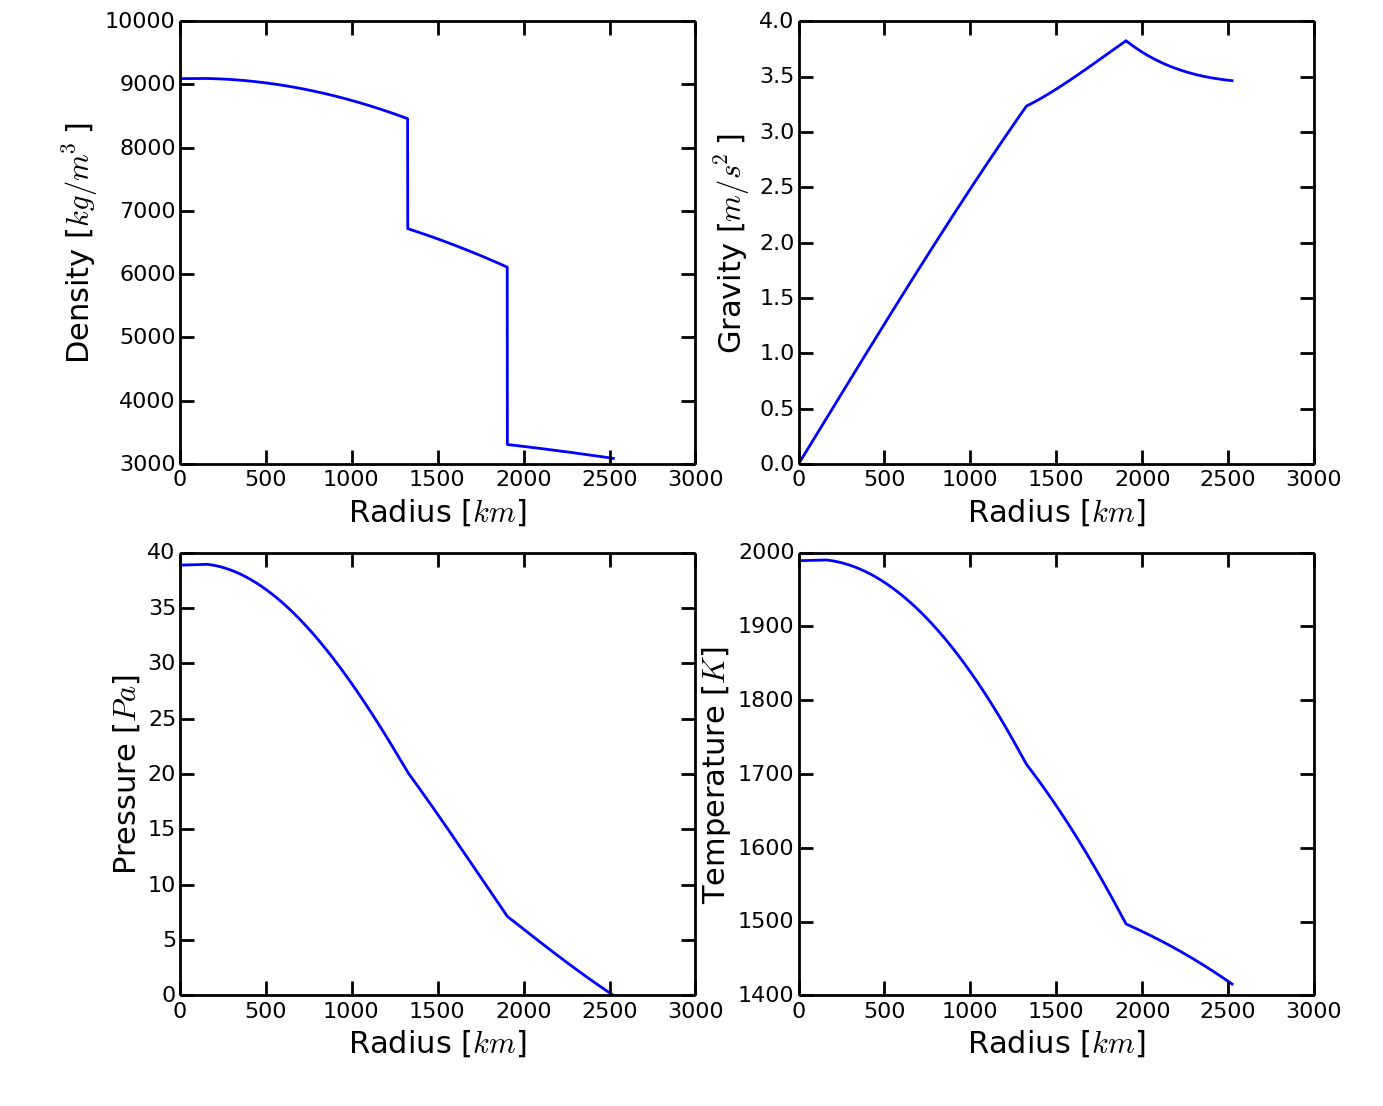
\includegraphics[width=0.165\textwidth]{profiles.png} &
 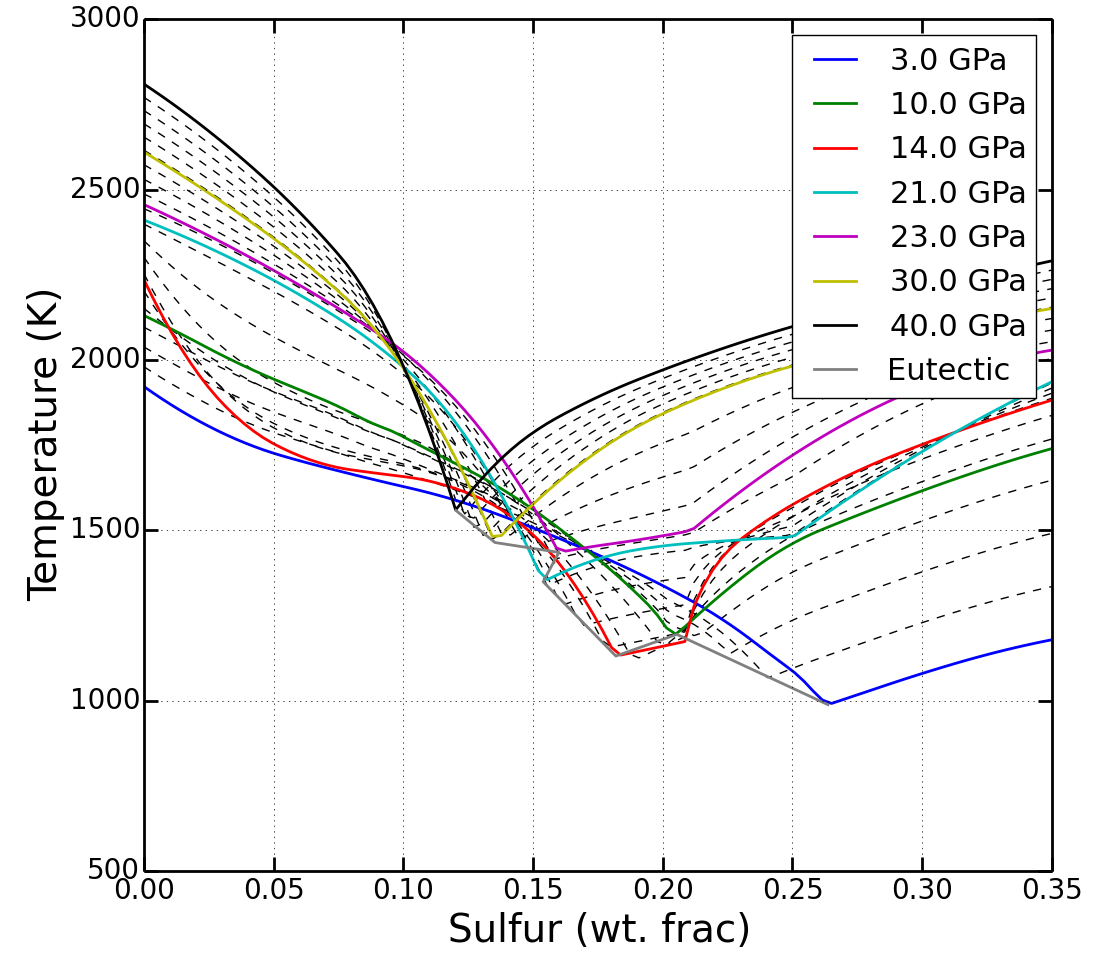
\includegraphics[width=0.15\textwidth]{Liquidus_model.png} \\
\end{tabular}
\captionof{figure}{Left: pressure, gravity, density, and temperature profiles of a reasonable interior model for Mercury.  Right: Liquidus curves for different pressures in the Fe-FeS system, from compiled and interpolated experimental data (Wicks and Knezek, pers. comm.) }
\label{interior_model}
\end{center}

Comparing the slope of the interpolated melting temperature to the slope of the
adiabatic profile determines the crystallization behavior of the core, with a
steeper melting temperature corresponding to  ``Earth-like'' conditions. For higher
values of the thermal expansivity, $\alpha$, the core will be ``snowing'' at all
times. For lower $\alpha$, the onset of snowing occurs with increasing S-content.

\columnbreak

\begin{center}
\begin{tabular}{cc}
 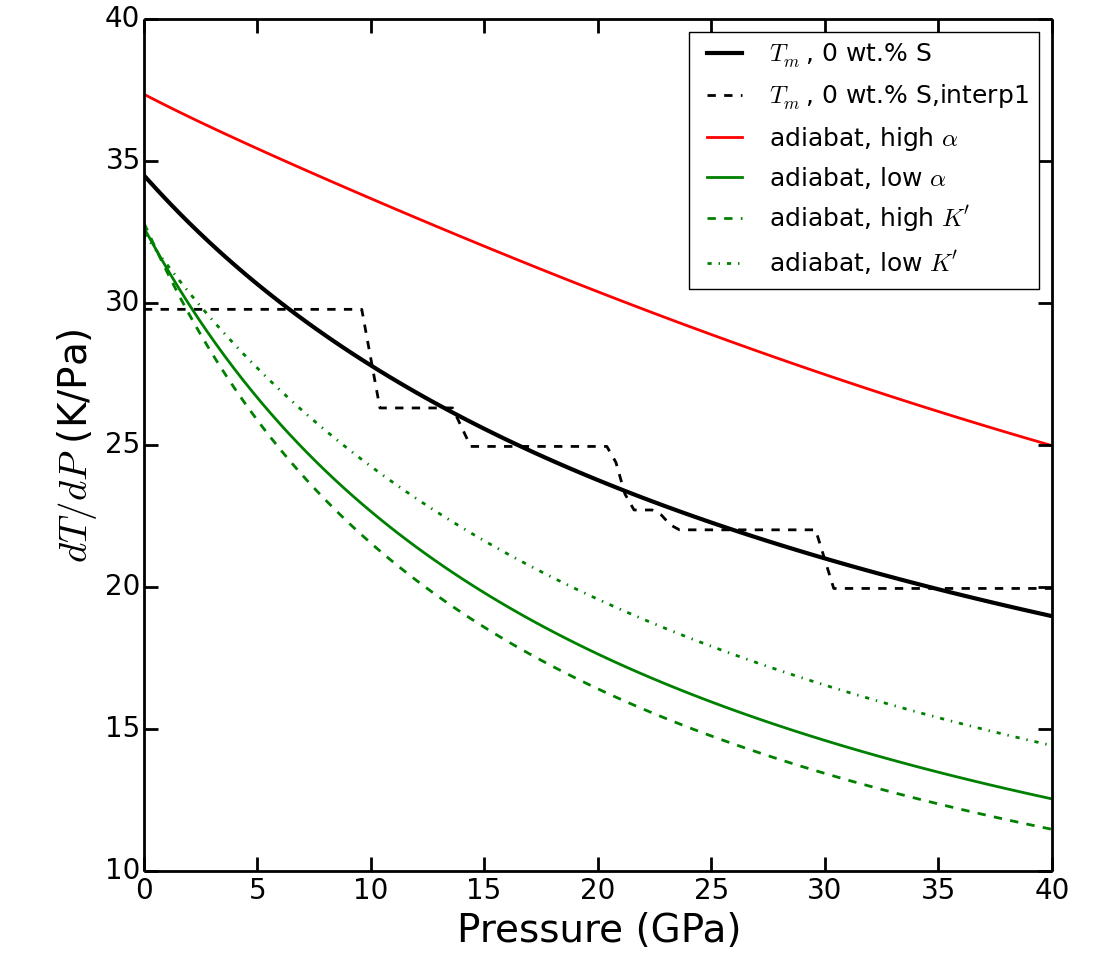
\includegraphics[width=0.15\textwidth]{clapeyron_1.png} &
 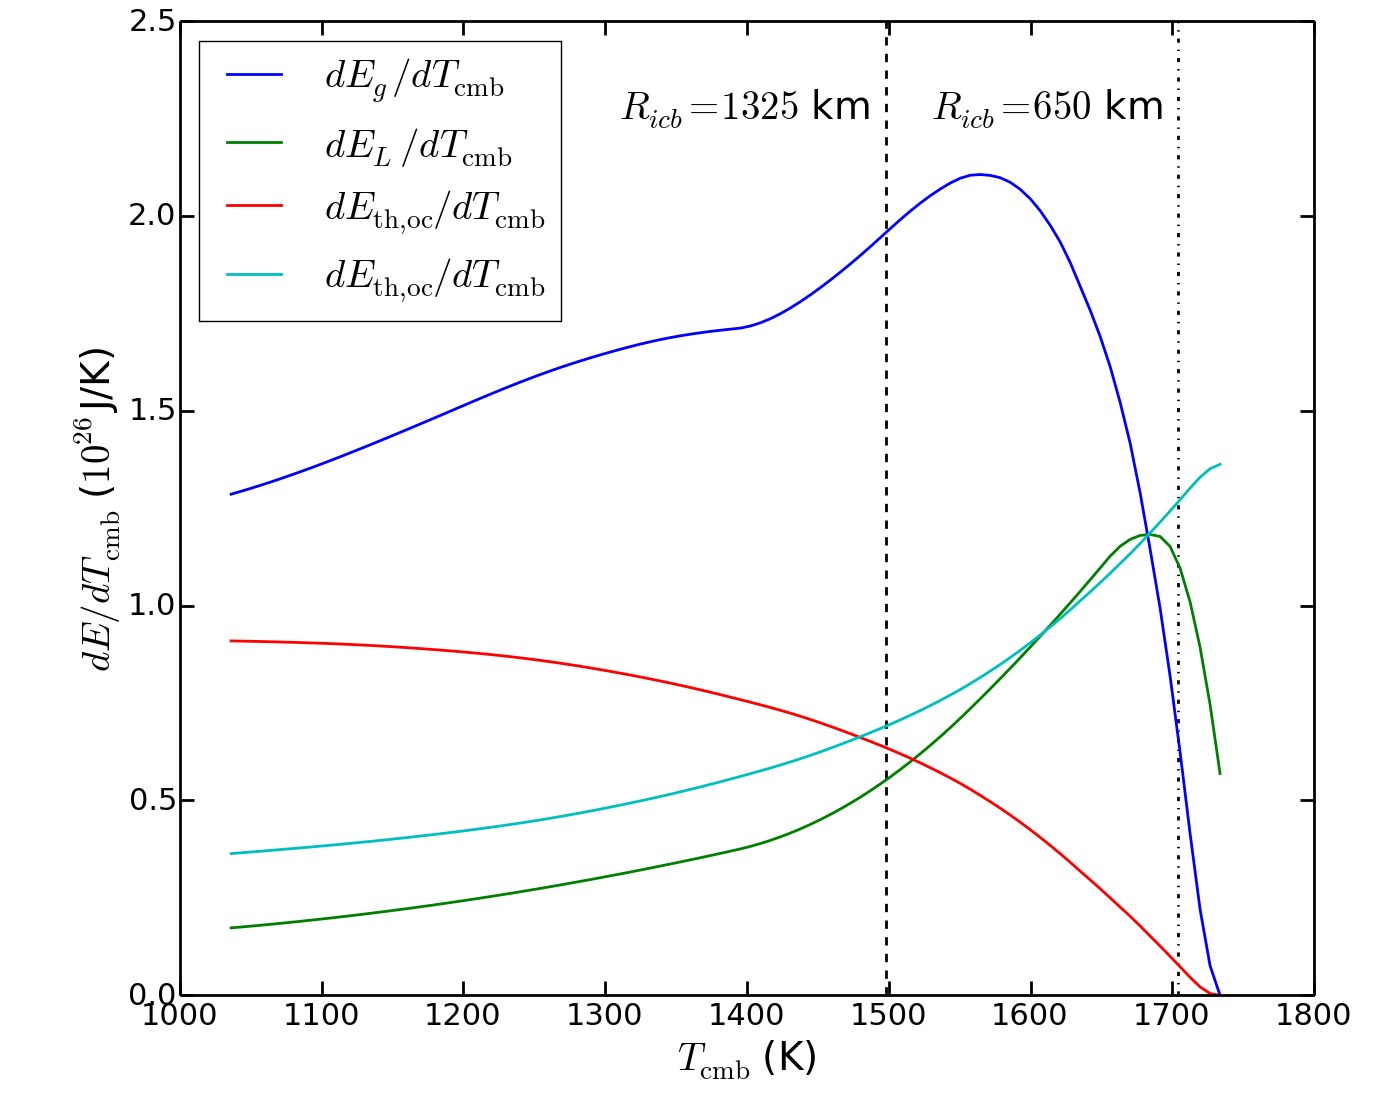
\includegraphics[width=0.165\textwidth]{core_energetics.png} \\
\end{tabular}
\captionof{figure}{Left: Clapeyron slopes and adiabats for different core models.  Right: resulting models for latent heat and gravitational energy release from a solidifying core. }
\label{core_energy}
\end{center}




The interior structure model can be coupled to a parameterized convetion model for
the thermal evolution of the planet. Shown on the right in Figure \ref{core_energy}
are the changes in latent heat, gravitational and thermal energy in the core per
change in core mantle boundary temperature for bulk composition of 6 wt.\% S. 

\section*{Parameterized convection and thermal evolution}



\begin{center}
\begin{tabular}{cc}
 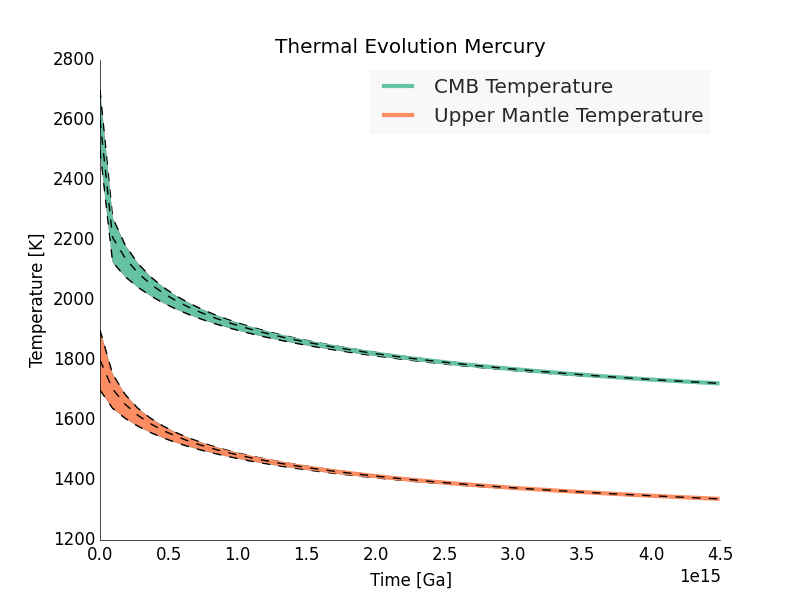
\includegraphics[width=0.15\textwidth]{thermal_evolution.png}
 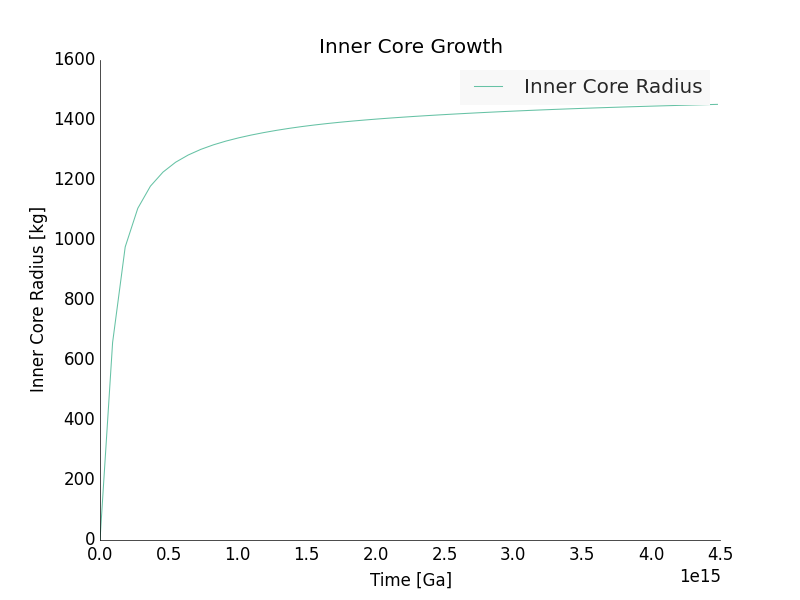
\includegraphics[width=0.15\textwidth]{inner_core_growth.png}
\end{tabular}
\captionof{figure}{Left: Thermal evolution of the Mercurian mantle and core. This thermal evolution model couples the core thermodynamics in the previous section with the mantl parameterization of Stevenson et al (1983). The colored regions show the solution for models with $\pm \mathrm{100}$ degress C. Note the break in slope of the $\mathrm{T_cmb}$ temperature with the onset of inner core growth at $\sim 2.5e2 Ma$. Right: Growth of the Inner Core versus time. This model run yields an inner core of $ \sim 1400 km$, slightly exceeding the upper bound of inner core size as constrained by Dumberry et al (2014).}
\label{flux}
\end{center}


\begin{center}
\begin{tabular}{c}
 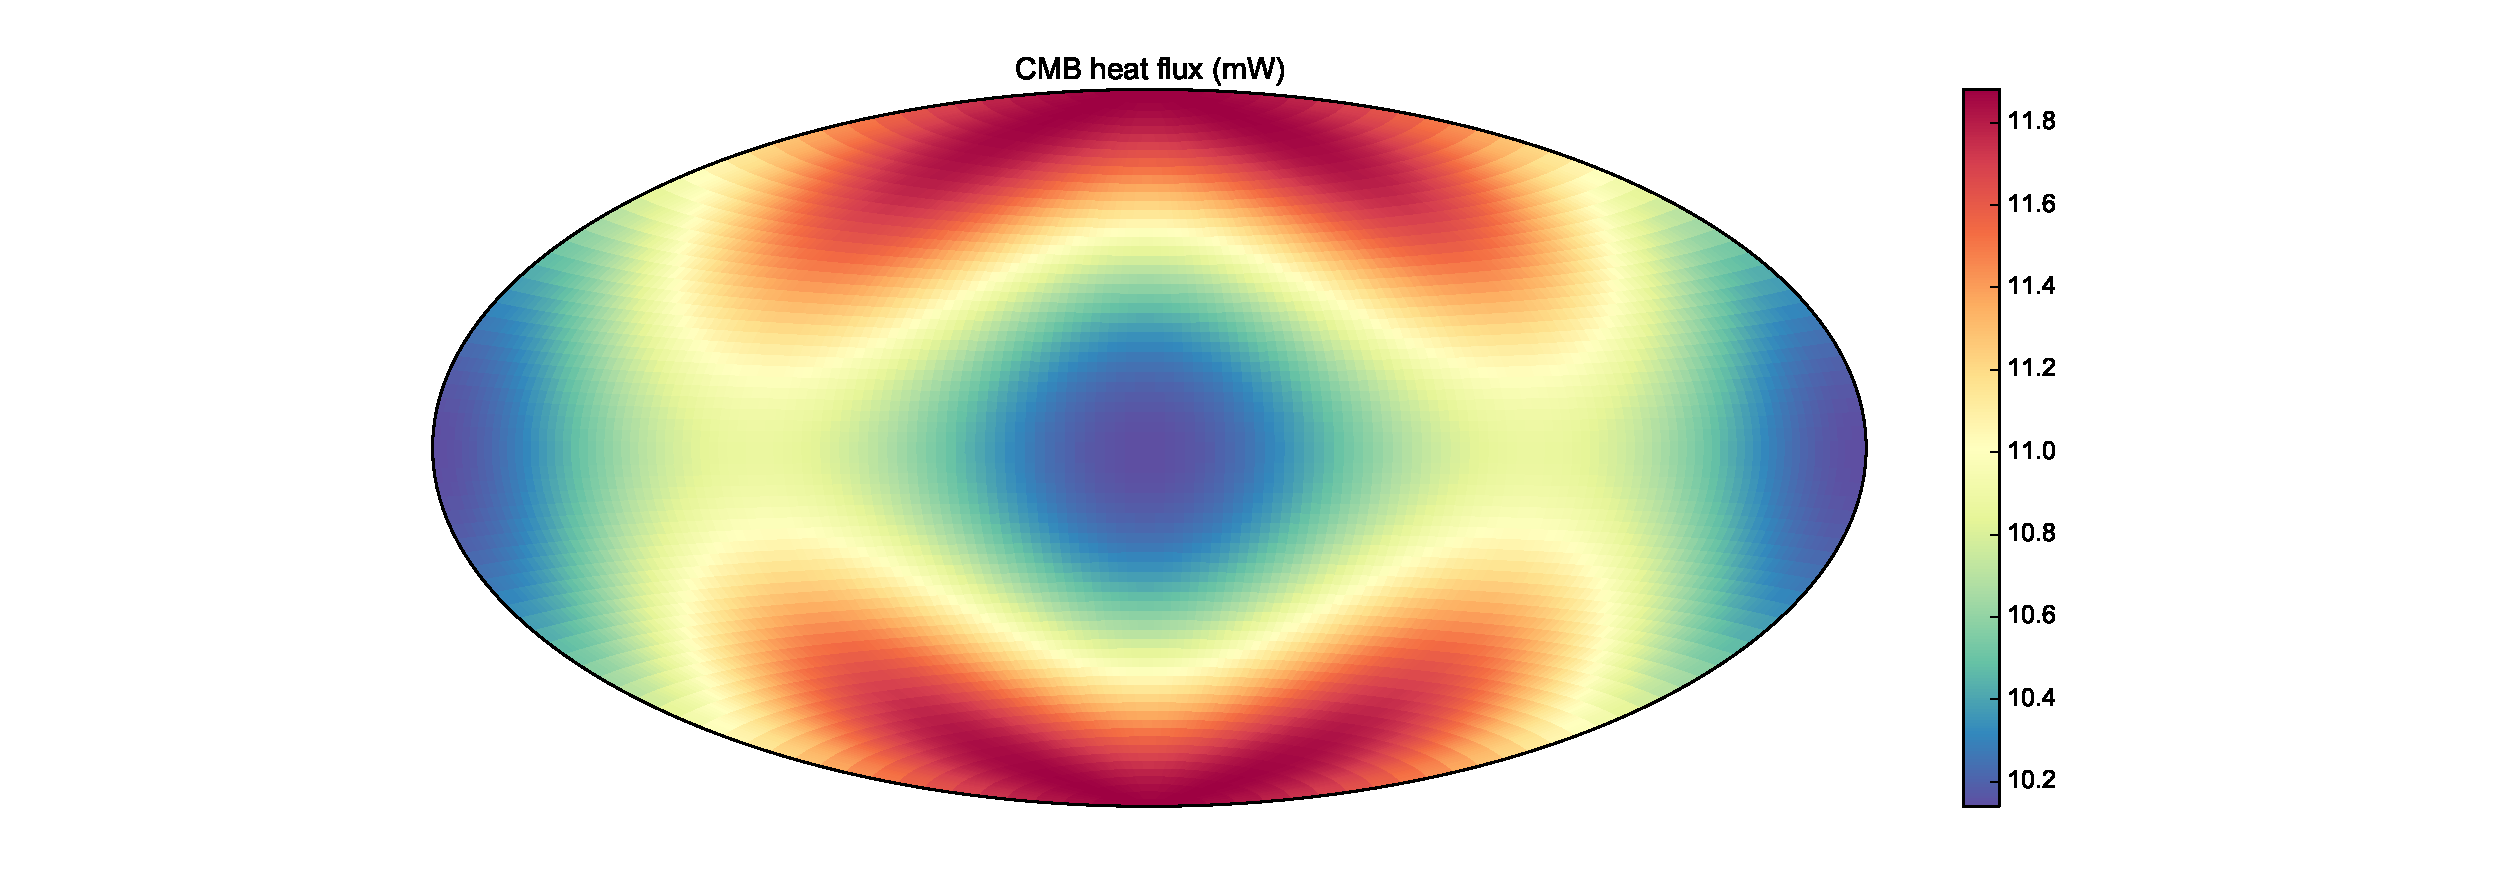
\includegraphics[width=0.18\textwidth]{CMB_flux.pdf} 
\end{tabular}
\captionof{figure}{ Heat flux variations for a conducting mantle with negligible internal heating. The total CMB heat flux is $\sim 0.6 \mathrm{TW}$, and peak-to-peak variations are about 20\%. }
\label{flux}
\end{center}

Mercury's unusual 3:2 spin-orbit resonance causes persistent temperature variations at the surface.  This boundary condition may create significant heat-flux variations at the CMB, especially if the mantle is not convecting.  Here we solve a simple conduction equation in the mercurian mantle to calculate an estimate of heat flux at the CMB.  This heat-flux variation is then used to inform the boundary conditions of a dynamo simulation using the \texttt{Calypso} code.

\columnbreak

\section*{Dynamo simulation}

We model a thermally driven dynamo in a rotating spherical shell with $r_{i}/r_{o} = 0.35$ (i.e.  $r_i$ = 700km).  The dynamo is driven with a non-dimensional heat flux $\mathrm{Nu} \sim 5$.  We test three cases for the heat-flux boundary condition: (1) homogeneous heat flux, (2) variations in the heat flux are scaled to be the same as the conducting-mantle variations, and (3) the variations in heat flux are scaled to be the ten times the conducting-mantle variations.
\begin{center}
\begin{tabular}{cc}
 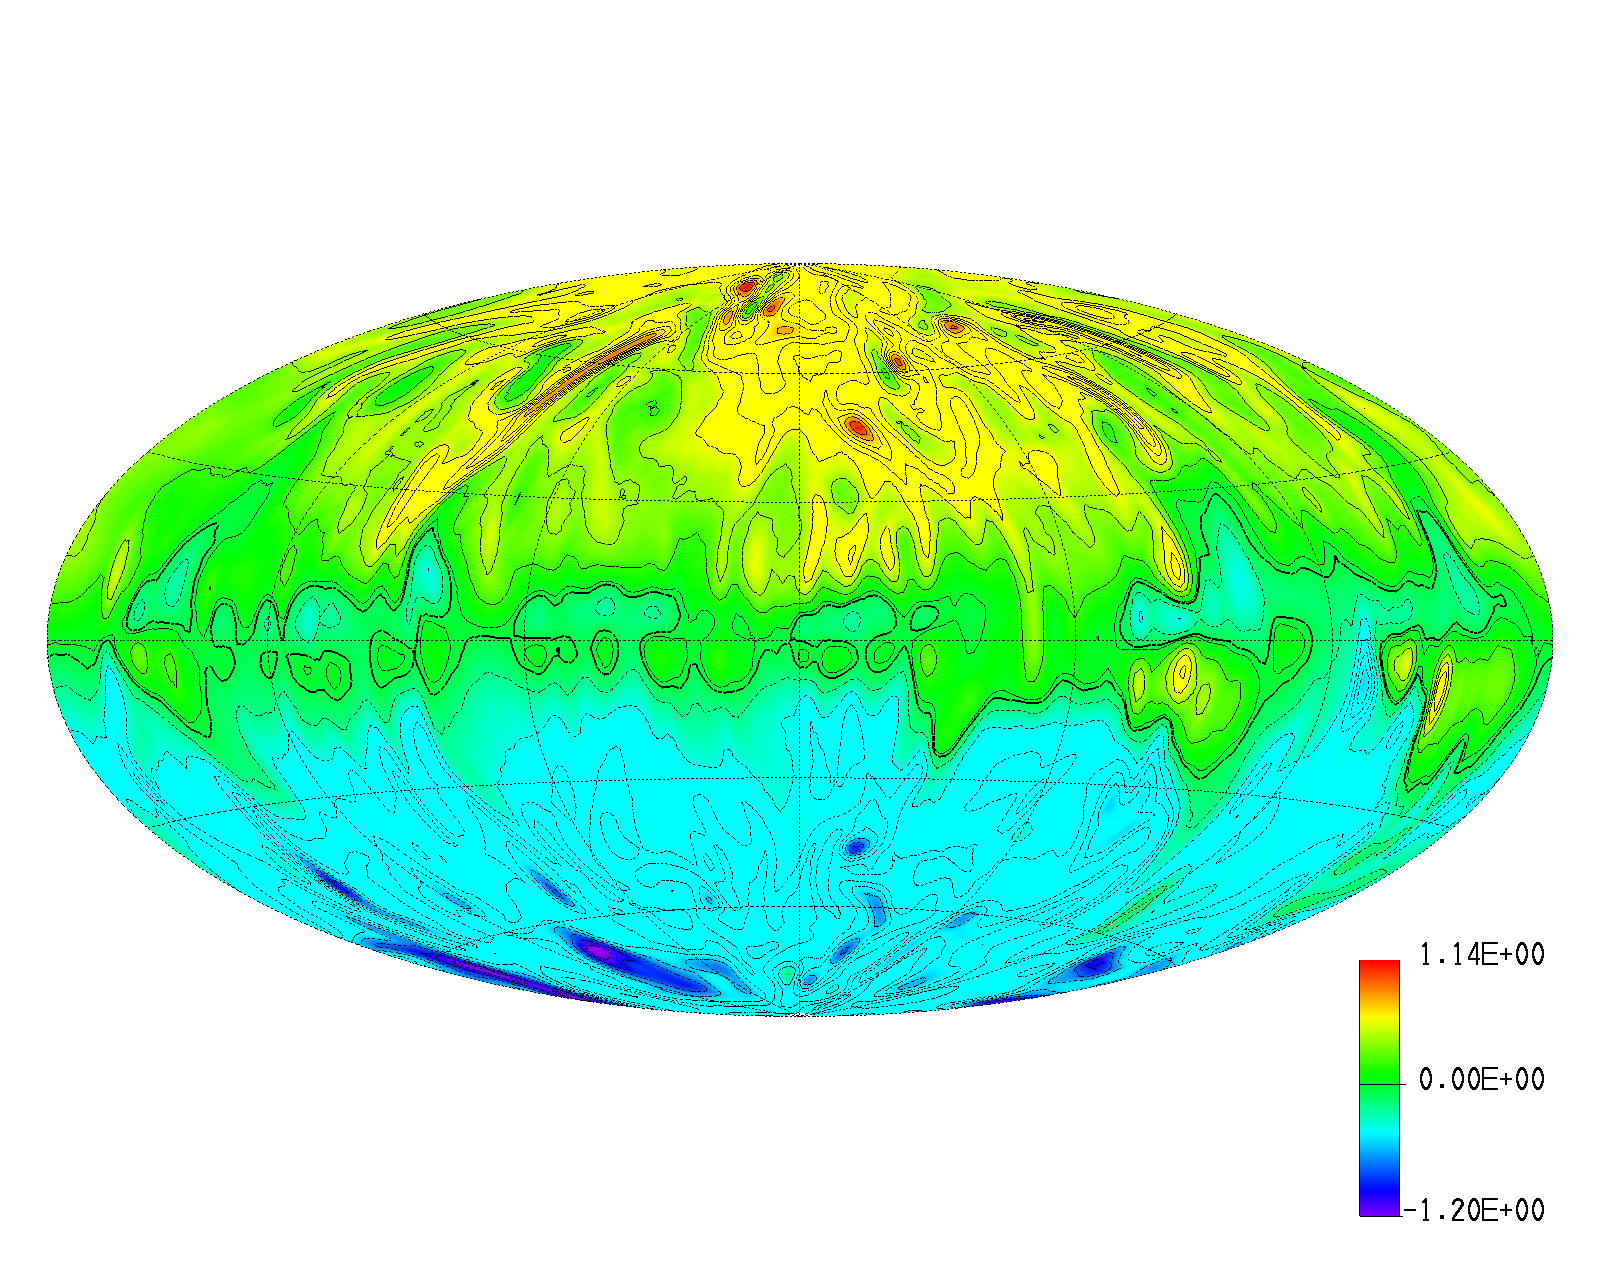
\includegraphics[width=0.1\textwidth]{br_cmb_x0.png} &
 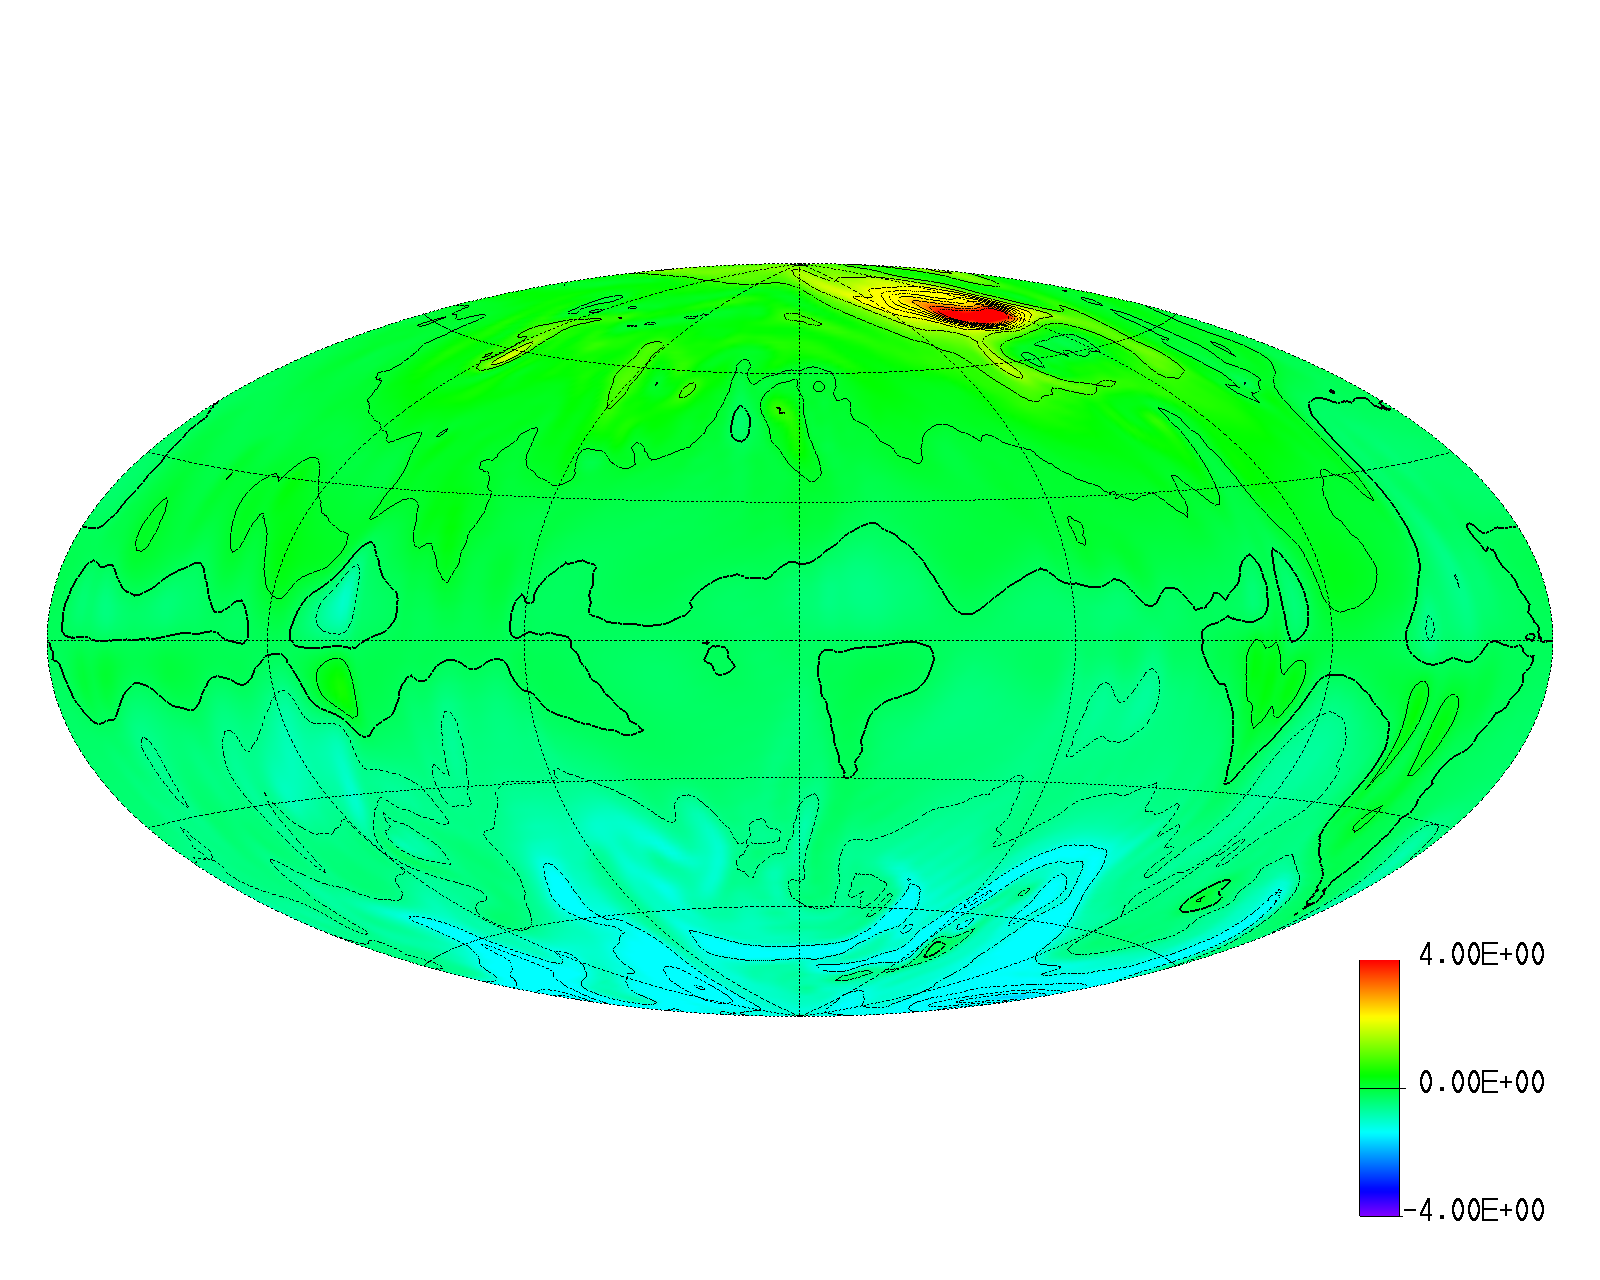
\includegraphics[width=0.1\textwidth]{br_cmb_x10.png}
\end{tabular}
\captionof{figure}{ Right: radial magnetic field at the CMB for the case of ten times larger heat flux heterogeneity case (case 3). Left: radial magnetic field in the homogeneous heat flux case (case 1).}
\label{dynamo}
\end{center}

\begin{center}
\begin{tabular}{c}
 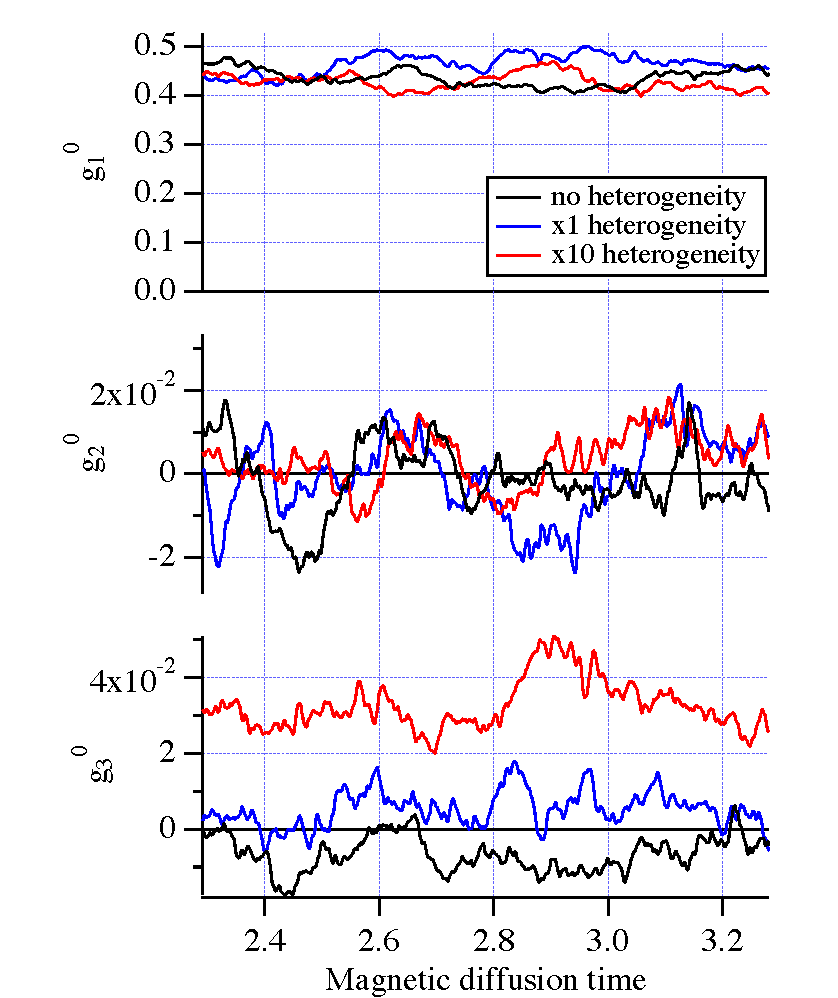
\includegraphics[width=0.15\textwidth]{gauss_coefficients.pdf} 
\end{tabular}
\captionof{figure}{ Time evolution of the first three axisymmetric components of Gauss coefficients at Mercury's surface. A significant difference is only observed in the $g_{3}^{0}$ component, which relects the position of intense patch (see \ref{dynamo}, right). }
\label{gauss}
\end{center}


To summarize preliminary results from our dynamo simulations:
\begin{itemize}
\item Large heat fluxes at the poles induce intense magnetic fields inside of tangent cylinder.
\item This magnetic patch is not stable in the present parameter regime.
\item The obtained magnetic field is larger than in the homogeneous heat flux case in the dipolar regime. The present solution may be too strong to explain the mercury's magnetic field.
\end{itemize}

{ \large Acknowledgements \\ \small
This project was initiated at the 2014 CIDER summer program.  We are grateful for continuing support from CIDER- NSF: 1135452.
Data for the Fe-FeS liquidus model was compiled and interpolated by June Wick and Nick Knezek.
We are grateful for helpful discussions with Bruce Buffett, Chris Davies, Mathieu Dumberry, and numerous CIDER participants.
}
\\
{ \large References \\ \tiny
Cottaar, Heister, Rose, and Unterborn. "BurnMan: A lower mantle mineral physics toolkit." Geochemistry, Geophysics, Geosystems 15.4 (2014): 1164-1179. \\
M. Dumberry and A. Rivoldini, Mercury’s inner core size and core-crystallization regime, Icarus, 248, 254-268 (2015). \\
Grott, M., D. Breuer, and M. Laneuville. "Thermo-chemical evolution and global contraction of Mercury." Earth and Planetary Science Letters 307.1 (2011): 135-146. \\
Hauck, Steven A., and Roger J. Phillips. "Thermal and crustal evolution of Mars." Journal of Geophysical Research: Planets (1991–2012) 107.E7 (2002): 6-1. \\
Matsui, Hiroaki, Eric King, and Bruce Buffett. "Multiscale convection in a geodynamo simulation with uniform heat flux along the outer boundary." Geochemistry, Geophysics, Geosystems 15.8 (2014) \\
Morschhauser, A., M. Grott, and D. Breuer. "Crustal recycling, mantle dehydration, and the thermal evolution of Mars." Icarus 212.2 (2011): 541-558. \\
Williams, Quentin. "Bottom-up versus top-down solidification of the cores of small solar system bodies: Constraints on paradoxical cores." Earth and Planetary Science Letters 284.3 (2009): 564-569.
 }

\end{multicols}


\end{document}

